\hypertarget{domain-background}{%
\section{Domain Background}\label{domain-background}}

One of the principal steps in the machine learning process is the
feature engineering\cite{sarkar2017practical}. It falls into the Data
Preparation step in the CRISP-DM, which is usually the most time
consuming (60\%\textasciitilde70\% of time in overall
project)\cite{sarkar2017practical}. In feature engineering there are two
different approaches: \textbf{feature selection} and \textbf{feature
extraction}\cite{sarkar2017practical}. Principal Component Analysis
(PCA) is a process of feature extraction\cite{sarkar2017practical} to
reduce the dimensionality of the data by understanding the individual
significance for a feature on the result of the
outcome\cite{shlens2014tutorial}. If two features are directly related
and change at the same rate, then there is no need to have both of them
to predict the output. For instance, if there are two features which
measure a phenomenon, one in meters and another one in inches, they are
measuring the same thing but in different scales. So there would only be
need to keep one of them.

\hypertarget{problem-statement}{%
\section{Problem Statement}\label{problem-statement}}

Alongside to competing in the \emph{Udacity+Arvato: Identify Customer
Segments Kaggle Competition}\cite{arvato_kaggle_competition}, this
project aims to compare the accuracy performance of the model with and
without applying the Principal Component Analysis techinque for
reduction of dimensionality. The goal of the competition is to help a
mail-order company, which sells organic products, to increase efficiency
in the customer acquisition process. To figure out which people in
Germany are most likely to be new customers, the attributes of existing
clients are analyzed and matched against a bigger data set that includes
attributes for people in the country.

Furthermore, it is expected that the PCA technique will improve the time
to train the model and also improve the accuracy prediction of the
model. This project will compare by how much the performance is
increased by applying the PCA techinque.

\hypertarget{datasets-and-inputs}{%
\section{Datasets and Inputs}\label{datasets-and-inputs}}

The data set used in this project will be the Arvato's data set provided
by the course in the Kaggle Competition\cite{arvato_kaggle_competition},
The Arvato's data set is a compilation of financial data from their
customers. The customers data set has 369 features (columns) and almost
200000 observations (rows), whereas the Germany data set contains 366
features (columns) almost 900000 observations (rows). The additional
features from the customers data set are: customer\_group,
online\_purchase, and product\_group. On listing \ref{lst:add_feat} is a
sample of those different features.

\begin{listing}[htp]
  \inputminted{python}{code/sample_additional_features.py}
  \caption{Sample of Additional Features}
  \label{lst:add_feat}
\end{listing}

\hypertarget{solution-statement}{%
\section{Solution Statement}\label{solution-statement}}

The model after having done the Principal Component Analysis will have a
better performance when training and predicting the possible customers.

\hypertarget{evaluation-metrics}{%
\section{Evaluation Metrics}\label{evaluation-metrics}}

We will train the model without applying any PCA technique and measure
the time it takes to train, the loss over epochs, the accuracy, fallback
and the other 2 (they relate false negative to overall negatives and so
on* search for these names)

Benchmark model, we will use a model without PCA and with PCA to compare
the solution.

\hypertarget{project-design}{%
\section{Project Design}\label{project-design}}

Download data, preprocess the data. All data should be between 0 and 1.
Fill empty cells with 0. Train with different hyperparameters. Train
with different number of cells per layer.

\hypertarget{reference}{%
\section{Reference}\label{reference}}

The materials that will be used as reference are the following:

\begin{itemize}
\item
  Article: A Tutorial on Principal Component Analysis by Jonathon Shlens
  (December 10, 2005; Version 2)
\item
  Book: Practical Machine Learning with Python: A Problem-Solver's Guide
  to Building Real-World Intelligente Systems by Dipanjan Sarkar, Raghav
  Bali, Tushar Sharma (2018)
\item
  Article: Customer Segmentation: Arvato Bertelsmann Project - A
  simplified technical report explaining my solution to building client
  profiles, targetting customers through demographics data, and
  communicating findings
  https://towardsdatascience.com/customer-segmentation-arvato-bertelsmann-project-44e73210a1b7
\end{itemize}

\hypertarget{andrew-ng---dimensionality-reduction}{%
\section{Andrew Ng - Dimensionality
Reduction}\label{andrew-ng---dimensionality-reduction}}

\hypertarget{data-compression}{%
\subsection{Data compression}\label{data-compression}}

Allows to approximate the original by projecting to a reduced dimension.
Halfs the memory requirements to store data. More importantly, learning
algorithms to run faster.

Data preprocessing before PCA: feature scaling/mean normalization. Mean
of each feature:
\(\mu_j = \frac{1}{m} \displaystyle\sum^{m}_{i=1}x_j^{(i)}\) Replace
each \(x_j^{(i)}\) with \(x_j - \mu_j\) to make feature have zero mean.
If different scales, scale features to have comparable range of values.

Reduce data from \(n\)-dimensions to \(k\)-dimensions Compute the
covariance matrix:
\(\Sigma = \frac{1}{m}\displaystyle\sum_{i=1}^n(x^{(i)})(x^{(i)})^T\)
Compute eigenvectors of matrix \(\Sigma\)

\(\Sigma\) is \(n \times n\) matrix. \((x^{(i)})\) is \(n \times 1\)
vector and \((x^{(i)})^T\) is \(1 \times n\) vector.

\([U,S,V] = svd(\Sigma)\)

\begin{align*}
X =
\left[
\begin{array}{ccc}
- & {x^1}^T & -\\
  & \vdots &   \\
- & {x^m}^T & - \\
\end{array}
\right]
\rightarrow \Sigma = \frac{1}{m} \times X^T \times X
\end{align*}

Output of \(svd\) are three matrices: \(U\), \(S\), and \(V\). \(U\) is
a \(n \times n\) matrix, where each column is the vector \(u^{(i)}\).

\begin{align*}
U = \left[
\begin{array}{cccccc}
\textpipe & \textpipe &        & \textpipe &        & \textpipe\\
u^1       &       u^2 & \cdots & u^k       & \cdots & u^n\\
\textpipe & \textpipe &        & \textpipe &        & \textpipe
\end{array}
\right]
\in \mathbb{R}^{n \times n}
\end{align*}

\(x\in\mathbb{R}^n\rightarrow z\in\mathbb{R}^k\)

\begin{align*}
U_{reduce} = \left[
\begin{array}{cccc}
\textpipe & \textpipe & & \textpipe\\
u^1 & u^2 & \cdots & u^k\\
\textpipe & \textpipe & & \textpipe
\end{array}
\right]
\in \mathbb{R}^{n \times k}
\end{align*}

Take the first \(k\) vectors to reduce to \(k\) dimensions.

\begin{align*}
Z &= U_{reduce}^T x\\
  &= \left[
\begin{array}{cccc}
- & u^1 & -\\
- & u^2 & -\\
  & \vdots &   \\
- & u^k & - \\
\end{array}
\right]
x
\end{align*}

Where \(U_{reduce}^T\) is \(k \times n\) and \(x\) is \(n \times 1\)

Choosing \(k\) (number of principal components)

Average squared projection error:
\(\frac{1}{m} \sum^m_{i=1} ||x^{(i)} - x_{approx}^{(i)}||^2\)

Total variation in the data: \(\frac{1}{m} \sum^m_{i=1} ||x^{(i)}||^2\)

Typically, choose \(k\) to be smallest value so that: \begin{align*}
\frac
{\frac{1}{m} \sum^m_{i=1} ||x^{(i)} - x_{approx}^{(i)}||^2}
{\frac{1}{m} \sum^m_{i=1} ||x^{(i)}||^2} \leq 0.01
\end{align*}

"99\% of variance is retained"

\hypertarget{algorithm}{%
\subsubsection{Algorithm}\label{algorithm}}

Try PCA with \(k=1\):

\textbf{Compute}

\(U_{reduce},z^{(1)},z^{(2)},\dots,z^{(m)},x^{(1)}_{approx},\dots,x^{(m)}_{approx}\)

\textbf{Check if}

\begin{align*}
\frac
{\frac{1}{m} \sum^m_{i=1} ||x^{(i)} - x_{approx}^{(i)}||^2}
{\frac{1}{m} \sum^m_{i=1} ||x^{(i)}||^2} \leq 0.01
\end{align*}

\([U,S,V] = svd(\Sigma)\)

The \(S\) matrix is a diagonal square matrix \(n \times n\):

\begin{align*}
S = \left[
\begin{array}{ccc}
s_{11}   &        & \bigzero \\
         & \ddots &          \\
\bigzero &        & s_{nn}   \\
\end{array}
\right]
\end{align*}

\begin{align*}
\frac
{\frac{1}{m} \sum^m_{i=1} ||x^{(i)} - x_{approx}^{(i)}||^2}
{\frac{1}{m} \sum^m_{i=1} ||x^{(i)}||^2} = 1 -
\frac
{\sum_{i=1}^k S_{ii}}
{\sum_{i=1}^n S_{ii}}
\end{align*}

\begin{align*}
\frac
{\sum_{i=1}^k S_{ii}}
{\sum_{i=1}^n S_{ii}}
\geq 0.99
\end{align*}

\hypertarget{supervised-learning-speedup}{%
\subsubsection{Supervised Learning
Speedup}\label{supervised-learning-speedup}}

\((x^{(1)},y^{(1)}),(x^{(2)},y^{(2)}),\dots,(x^{(m)},y^{(m)})\)

\(x^{(i)}\in\mathbb{R}^{10,000}\)

\begin{align*}
x^{(1)}, x^{(2)},& \dots, x^{(m)}, \in\mathbb{R}^{10,000}\\
&\downarrow \text{PCA}\\
z^{(1)}, z^{(2)},& \dots, z^{(m)}, \in\mathbb{R}^{1,000}\\
\end{align*}

New training set

\((z^{(1)},y^{(1)}),(z^{(2)},y^{(2)}),\dots,(z^{(m)},y^{(m)})\)

Hypothesis

\begin{align*}
h_{\uptheta}(z) = \frac{1}{1+e^{-\uptheta^{T}z}}
\end{align*}

If you have new example, take x, map throug the same PCA to get the
corresponding z, and then z can

What PCA does is mapping \(x^{(i)} \rightarrow z^{(i)}\). This should be
done only on the training set. This mapping can be applied as well to
examples \(x^{(i)}_{cv}\) and \(x^{(i)}_{test}\) in the cross validation
and test sets.

\hypertarget{bad-us-of-pca-to-prevent-overfitting}{%
\subsection{Bad us of PCA: To prevent
overfitting}\label{bad-us-of-pca-to-prevent-overfitting}}

Use \(z^{(i)}\) instead of \(x^{(i)}\) to reduce the number of features
to \(k<n\). Thus, fewer features, less likely to overfit.

Not a good way to address overfitting. Use regularization instead.

\begin{align*}
\min_{\theta} \frac{1}{2m} \sum^{m}_{i=1}(h_{\theta}(x^{(i)}) - y^{(i)})^2 + \frac{\lambda}{2m}\sum^{n}_{j=1}\theta^2_j
\end{align*}

Regularization uses the labels, whereas PCA don't and might throw away
valuable information.

\hypertarget{uses-where-it-shouldnt-be}{%
\subsubsection{Uses where it shouldn't
be}\label{uses-where-it-shouldnt-be}}

Design of ML system:

\begin{itemize}
\item
  Get training set
  \((x^{(1)},y^{(1)}),(x^{(2)},y^{(2)}),\dots,(x^{(m)},y^{(m)})\)
\item
  Run PCA to reduce \(x^{(i)}\) in dimension to get \(z^{(i)}\)
\item
  Train logistic regression on
  \((z^{(1)},y^{(1)}),\dots,(z^{(m)},y^{(m)})\)
\item
  Test on test set: Map \(x^{(i)}_{test}\) to \(z^{(i)}_{test}\).
\item
  Run \(h_{\uptheta}(z)\) on on
  \((z^{(1)}_{test},y^{(1)}_{test}),\dots,(z^{(m)}_{test},y^{(m)}_{test})\)
\end{itemize}

How about doint the whole thing without using PCA?

Before implementing PCA, first try running whatever you want to do with
the original/raw data \(x^{(i)}\). Only if that doesn't do what you
want, then implement PCA and consider using \(z^{(i)}\).

\hypertarget{a-tutorial-on-principal-component-analysis}{%
\section{A Tutorial on Principal Component
Analysis}\label{a-tutorial-on-principal-component-analysis}}

\cite{shlens2014tutorial}

Principal component analysis (PCA) is a simple, non-parametric method of
extracting relevant information from confusing data sets. With minimal
additional effort PCA provides a roadmap for how to reduce a complex
data set to a lower dimension on reveal the sometimes hidden, simplified
structure that ofter uderlies it.

PCA is intimately related to the mathematical technique of singular
value decomposition (SVD). Assimptions and limitations?

\hypertarget{framework-change-of-basis}{%
\subsection{Framework: Change of
Basis}\label{framework-change-of-basis}}

The goal of principal component analysis is to compute the most
meaningful basis to re-express a noisy data set. The hope is that this
new basis will filter out the noise and reveal hidden structure.
Determining this fact allows an experimenter to discern which dynamics
are importante, which are just redundant and which are just noise.

\hypertarget{diagonalize-the-covariance-matrix}{%
\subsection{Diagonalize the Covariance
Matrix}\label{diagonalize-the-covariance-matrix}}

Select a normalized direction in m-dimensional space along which the
variance in X is maximeizes. Save this vector as p1. Find another
direction along which variance is maximized, however, because of the
orthonormality condition, restrict the search to all directions
perpindicular to all previous selected directions. Save this vector as
pi. Repeate this procedure until m vectors are selected.

The resulting ordered set of p's are the \emph{principal components}.

The variances associated with each direction pi quantify how "principal"
each direction is.

\hypertarget{a-more-general-solution-svd}{%
\subsection{A more general solution:
SVD}\label{a-more-general-solution-svd}}

Singular Value Decomposition (SVD) is a more general method of
understanding change of basis

\hypertarget{discussion-and-conclusions}{%
\subsection{Discussion and
Conclusions}\label{discussion-and-conclusions}}

\hypertarget{quick-summary}{%
\subsubsection{Quick Summary}\label{quick-summary}}

Performing PCA is quite simple in practice

\begin{enumerate}
\def\labelenumi{\arabic{enumi}.}
\item
  Organize a data set as an \emph{m} x \emph{n} matrix, where \emph{m}
  is the number of measurement types and \emph{n} is the number of
  trials
\item
  Subtract off the mean for each measurement type of row \textbf{xi}.
\item
  Calculate the \emph{SVD} or the eigenvectors of the covariance.
\end{enumerate}

In several fields of literature, many authors refer to the individual
measurement types \textbf{xi} as the \emph{sources}. The data projected
into the principal componentes \textbf{Y = PX} are termed the
\emph{signals}, because the projected data presumably represent the
underlying items of interest.

\hypertarget{dimensional-reduction}{%
\subsubsection{Dimensional Reduction}\label{dimensional-reduction}}

One benefit of \emph{PCA} is that we can examine the variance
\textbf{Cy} associated with the principle components. Often one finds
that large variances associated with the first \emph{k} \textless{}
\emph{m} principal components, and then a precipitous drop-off. One can
conclude that most interesting dynamics occur only in the first \emph{k}
dimensions.

This process of throwing out the less important axes can help reveal
hidden, simplified dynamics in high dimensional data. This process is
aptly named \emph{dimensional reduction}.

\hypertarget{udacity-15.-pca-overview}{%
\section{Udacity 15. PCA, Overview}\label{udacity-15.-pca-overview}}

Principal Component Analysis (PCA) attempts to reduce the number of
features within a dataset while retaining the ``principal components'',
which are defined as weighted combinations of existing features that:

Are uncorrelated with one another, so you can treat them as independent
features, and Account for the largest possible variability in the data!
So, depending on how many components we want to produce, the first one
will be responsible for the largest variability on our data and the
second component for the second-most variability, and so on. Which is
exactly what we want to have for clustering purposes!

PCA is commonly used when you have data with many many features.

You can learn more about the details of the PCA algorithm in the video,
below.

The idea is that components that cause a larger variance will help us to
better differentiate between data points and (therefore) better separate
data into clusters.

So, next, I'll go over how to use SageMaker's built-in PCA model to
analyze our data.

\hypertarget{transcripts}{%
\subsection{Transcripts}\label{transcripts}}

\hypertarget{pca-toy-problem-sc-v1---lang_en.srt}{%
\subsubsection{13 - PCA Toy Problem SC V1 -
lang\_en.srt}\label{pca-toy-problem-sc-v1---lang_en.srt}}

How to use principal component analysis for dimensionality reduction.
\textbf{Dimensionality reduction}, is one of the main applications of
PCA. \textbf{In the previous lessons}, you've already learned how PCA
works and about eigenvectors and eigenvalues. \textbf{In this notebook},
we will see how to apply PCA to a small dataset.

Let's begin by understanding what dimensionality reduction is all about.
Let's suppose we had some two dimensional data that looks like the Fig.
\ref{fig:dimensionality_reduction}.

\begin{figure}[htp]
  \centering
  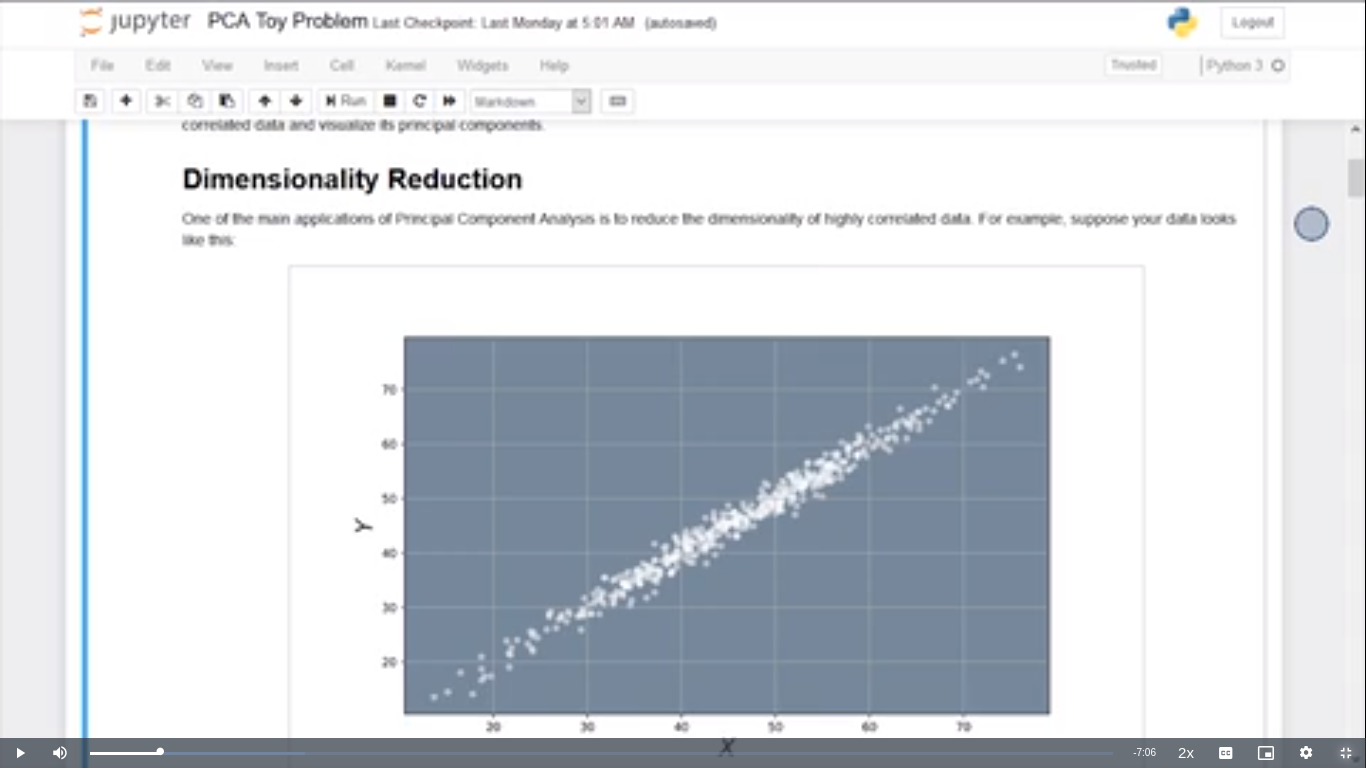
\includegraphics[width=\linewidth]{img/dimensionality_reduction.png}
  \caption{Dimensionality Reduction data}
  \label{fig:dimensionality_reduction}
\end{figure}

We can see that most of the data points lie close to a straight line. We
can also see that most of the variation in the data occurs along this
direction, but there's not much variation along this direction. This
means we can explain most of the variation of the data by only looking
at how the data points are distributed along this straight line.
Therefore, we could reduce this two-dimensional data to one-dimensional
data by projecting all these data points onto this straight line. By
projecting the data onto a straight line, we can actually reduce the
number of variables needed to describe the data because you only need
one number to specify a data point's position along a straight line.
Therefore, the two variables that describe the original data can be
replaced by a new variable that actually encodes this linear
relationship.

It is important to note that the new variable is just an abstract tool
that allows us to express this data in a more compact form, and may or
may not be interpreted as a real-world quantity. Now, let's see how we
can do this in code. For simplicity, we will use a small two-dimensional
dataset. In a later notebook, you'll get a chance to apply what you
learned in this notebook to real stock data. We will start by creating
some randomly correlated data. In this code, you can choose the range of
your data and the amount of correlation. The code outputs a plot with
the data points and the amount of correlation. In this case, we chose
our data range to be between 10 and 80. Therefore, the datapoints range
between 10 and 80 in both the x and y axis. Remember, a correlation of
zero means no correlation at all, and a correlation of one means
complete correlation. You can vary the amount of correlation and create
the data that you like. Once you have created your data, the next step
in PCA is to center your data around zero. It is also customary to
normalize your data. This is known as mean normalization. While
centering the data is necessary, normalizing the data is optional, and
this is what I have done here. Mean normalization not only centers your
data around zero, but also distributes your data evenly, in a small
interval around zero. As you can see here, the data is no longer in the
range between 10 and 80. But after normalization, the data is now
distributed between minus three and three. This will help your algorithm
converge faster. With our data centered, we're ready to perform PCA. To
do this, we will use a package called Scikit-learn. Scikit-learn's PCA
class allows us to easily implement PCA on data. The first thing we need
to do is to create a PCA object with a given set of parameters including
the number of principal components we want to use. We'll start by using
two components because we want to visualize them later. Here, we can see
the parameters that the PCA algorithm is going to use. The next step is
to pass the data to the PC object using the fit method. A quick note. In
Scikit-Learn, the PCA algorithm automatically centers the data for you.
So, you could pass the original dataset to the fit method instead of the
normalized data as we have done here. Once we fit the data, we can use
the attributes of the PCA class to see the eigenvectors also known as
the principle components, and its eigenvalues. One important attribute
of the PCA class is the explained variance ratio. The explained variance
ratio gives us the percentage of variance explained by each of the
principal components. In general, the principle components with the
largest eigenvalues explain the majority of the variance, and this is
usually the ones that we want to keep. For example, here we can see that
the first principle component explains 94 percent of the variance, and
has the largest eigenvalue. Now that we have the principle components,
we can visualize them. Here, we see the data with the first principle
component, and the second principle component. We can see that the first
principal component lies along the direction in which the data varies
the most. One question that you will frequently face is how many
principal components you should use. For example, suppose you had a
dataset with 1,000 dimensions. Should you reduce this dataset to 500
dimensions or could you do better and reduce it to 100 dimensions?
Usually, the number of principal components is chosen depending on how
much of the variance of the original data you want to retain. For
example, you may want to retain 90 percent of the variance, or you may
only want to retain 50 percent of the variance. You can use the
explained variance ratio attribute of the PCA class to determine the
number of components you need to keep to retain a given amount of
variance. For example, if you wanted to retain 90 percent of the
variance, you can add up the elements in the explained variance ratio
array until the desired value is reached. The number of elements you had
to add up to reach the desired value determines the number of principal
components needed to retain that level of variance. For example, if you
had to add up five elements to retain 90 percent of the variance, then
you will need five principal components. Now, that we have seen what all
the principal components look like, we will now use PCA to perform
dimensionality reduction. Since the data we're using in this simple
example only has two dimensions, the best we can do, is to reduce it to
one dimension. So, now choose the number of principle components in our
PCA algorithm to be equal to one. Once we ran the PC algorithm with only
one component, we can see what the transform data looks like by using
the transform method of the PCA class. In this simple case, the
transform method projects the data onto the first principal component so
we will just get a straight line. When working with higher dimensional
data, the transform method will project the data onto the
lower-dimensional surface determined by the number of principal
components you used in your algorithm.

\hypertarget{l1c8-pca-estimator-v2---lang_en.srt}{%
\subsubsection{14 - L1C8 PCA Estimator V2 -
lang\_en.srt}\label{l1c8-pca-estimator-v2---lang_en.srt}}

One thing to note is that each data point here has 34 associated
features. So this is 34 dimensional data which is pretty high
dimensional. Unsupervised algorithms rely on finding relationships in n
dimensional feature space. For higher dimensions, we often get noisier
clustering, for example. So an algorithm like K-means has a hard time
figuring out which dimensions to pay attention to. Some of these
dimensions are not as important as others. For example, if every county
in our dataset had the same exact total population, then this particular
feature wouldn't give us any distinguishing information. It would not
help us to separate the counties into different groups because its value
doesn't vary between counties. This is just a hypothetical example.
Instead, we really want to find the features that help us separate
ungrouped data. In other words, we want to find features that cause the
most variance in our dataset. So before we cluster this data with
K-means, I want to take one more step, a dimensionality reduction step.
My aim will be to form a smaller set of features that will better help
us separate our data. The technique we'll use is called PCA or Principal
Component Analysis. PCA is most useful when you have a bunch of features
and you want to find out which linear combinations of these features
matter the most, which are responsible for the largest variance in our
data. So to perform PCA, we'll use SageMaker's built-in model for PCA.
To create any model, you'll first need to specify an IAM role and
SageMaker session. Please let the model know what permissions and
session to train in. So in this cell here, I'm storing our SageMaker
session by calling sagemaker.Session. This is a capital S. It's a
session object, and I'm storing that as a variable here. Then, I am
getting the IAM role. We specified this role earlier, and I'm getting it
by name with an import get\_execution\_role. I'll actually print it out
to make sure it's the right name. So we have our session, and this role
name should look familiar from when we created the Notebook. Next, we'll
also need a place to store the trained model in an S3 bucket. So in this
next cell, I'm creating a default bucket from our SageMaker session with
a call to.default\_bucket, and I'm saving the name of that bucket for
reference later. If you print out the name of this default bucket, you
should get something like this. It says SageMaker, and then it has your
region, mine is US-West-1, and then some numbers to make it unique.
Then, I'll start to build a PCA model and I'll need to do a few things.
First, I'm going to specify exactly where, in our S3 bucket, I want to
store the trained model artifacts. I'll specify a prefix for a directory
where I want to store the data, calling it counties for data about
counties in the US. Here I'm creating the entire output path which is a
string that points to the bucket, and the prefix directory. Next, it's
time to define the PCA model. So this model is built-in in SageMaker and
I can import it by name, import PCA. Then, I'm creating a model down
here. I'm saving it as pca\_SM for SageMaker, and I'm calling our PCA
constructor here. This takes in several arguments. First, I'm passing in
the IAM role which we defined above. Then, I'm specifying the train
instance count, which will usually be one, and the instance type, which
I'm setting as a c4.xlarge. Then, I'll specify the output path as this
one that we defined above. Again, this is the place that the resultant
model data will be stored in S3. Then, I'm also passing in the SageMaker
session that we also just defined. Now, there's one last thing I need to
specify, and that is a hyperparameter for the PCA model. Basically, this
model needs to know how many principal components we want to create. We
want to reduce our 34 dimensions of data but we'll actually want to
first generate enough linearly independent principal components to
capture the variance in our data, and at later, select the top
components to pass to our clustering model. So I'll define N\_COMPONENTS
as 33. This is the existing feature dimension, 34, minus one. This is a
good rule of thumb for starting PCA analysis. So again, I'm going to
generate 33 of these principal components, but then, later, I'll select
only a few of the top components to use in our final clustering
algorithm. This is going to be in all caps because it's a global
variable. That means after defining it, I'll be able to access it in any
later cell in the Notebook. So let me recap how I create an estimator
like this. First, I'm going to import that built-in model from
SageMaker, and then this takes in a number of constructor parameters. It
takes in the role and SageMaker session which I got an a cell above,
here. They're default parameters that are accessible from our Notebook.
The session and role are variables that you can always get from your
Notebook instance. I also specified an output path which is where this
model will be saved after it trains in our S3 bucket. Then, I had to
specify the instance count and type for training. Lastly, our hyper
parameter for a PCA model, the number of components, 33, that we want to
generate. Okay. So I'm running the cell. Then, after defining this
model, I'll actually want to create a training job and train it on our
county's data. A requirement for all of SageMaker's built-in models is
that the passed-in training data be a record set. This allows training
of models within SageMaker to perform really fast compared to, say,
Scikit-learn models, especially for large datasets. So to get a record
set format, first, I'm going to convert our scale dataframe into a NumPy
array calling values.astype, float32. I'll save this NumPy array as
train\_data\_np. Then, I can actually call our model.record\_set and
pass in this NumPy data to create our formatted training data in a
record set format. So going from NumPy to record set, I get our
formatted train data. Finally, to train the model, I call pca\_SM.fit
and pass in this formatted train data. If I run this cell, this should
kick off a training job and I can see the name of that training job
here. This job will take a little while to complete, so I can show you a
few things while it runs. I'm actually going to go back to my Amazon
SageMaker console. Now, in all these buttons on the side, you'll see
this one for training jobs. When I click this, I can actually see the
PCA job that I just kicked off. It's in progress. I'll see a list of all
these other jobs that I've done in the past. But let's click on this
most recent one that's in progress. So in here, I can see the job name
and the IAM role that it's attached to. I can see that it's in progress
and read a bit about the details about this training job. If I scroll
all the way down to Monitor, I'll actually be able to click on the logs,
which will be really useful if I need to debug a training job if it's
failed, for example. The logs are where any errors and trace back will
be recorded. A failed job has happened to me a few times as I've
developed, and the key is just to read through the logs and debug.
Debugging is part of coding just like any other step. So I just wanted
to show you this option of how to explore more information about a
unique training job. Back to my Notebook, I can also see how the
training job is monitored in the Notebook itself. I'll see print
statements and timestamps that indicate when an instance is being spun
up, when import data is being downloaded, and some details about the
training in progress. Then, because I was timing this, at the end, I can
scroll down and see how long this whole process took a few minutes. Now
that this training job is complete, I have a trained model. Next, I'll
actually want to see the principle components that the model has come up
with. I want to see what linear combinations of features make up each
component and decide on the number of top components to include as I
create new reduced dimensionality training data.

\hypertarget{l1c9-pca-attributes-variance-v3---lang_en.srt}{%
\subsubsection{15 - L1C9 PCA Attributes Variance V3 -
lang\_en.srt}\label{l1c9-pca-attributes-variance-v3---lang_en.srt}}

We've just trained the PCA model and now we can access the underlying
model parameters. One thing that we'll need is the name of the training
job. I'm going to copy it from here, we could also get it from the AWS
console. Saved model artifacts are stored in S3 as a TAR file. This is a
compressed file in the output path that we specified in the location
output path, and it will also be saved in this output/model.tar.gz
extension. We can explore the artifacts that are stored here and use
them to deploy a trained model. So in here, I'm going to copy and paste
my training job name, and then the model key is going to be the prefix
counties that we specified earlier, this job name, and the output
extension. Then similar to how we downloaded the CSV file before, we're
going to pass in that model key, the bucket name, and call download file
on our boto3 resource. Then I actually have a couple more lines of code
that will unzip this compressed file and store it as model\_algo-1, this
name is consistent across models. So if this so executed, this should
print out the model key and some confirmation code. Now built-in
SageMaker models are built on something called MXNet. So I'm importing
this as a library mx, and this gives us certain tools to use. I'm going
to load in the parameters of our model by name, which is model\_algo-1.
The mx library allows me to load this in as an ndarray. I'm saving all
of these as the PCA model parameters and printing them out here. I can
see that this array holds three main values, s, v, and down here a mean
value, and I'll be able to access these arrays by name. I have some
explanations of what each of these is here. The mean is the mean that's
subtracted from a component in order to center it, this is part of the
PCA calculation. v is the makeup of the principal components, so which
linear combinations of original features make up each principal
component? s are the singular values of the components. Now, we talked
about getting components that will cause the most variance in our
dataset. s will not give us the exact percentage data variants, but it
can help us calculate a good approximation, according to this
approximate explained variance formula, which I'll go over in a bit. The
important thing to note is that, for looking at the principal components
and the data variance, we'll be interested in v and s only. I'm actually
going to load the specific parameters calling them by name, and loading
them in as DataFrames s and v here. So first, let's talk about s and the
data variance. I mentioned that from s, we can get an approximation of
the data variance that is explained in the first and principal
components. The approximate explained variance is given by this formula.
This is the sum of s squared for all selected top\_n components, over
the sum of squares for all components. Why are we interested in variants
in the first place? Why is variants so important? Well, the challenging
part of doing dimensionality reduction with PCA, is deciding on the
number of top components we want to get from our data, and eventual use
in our final clustering model. Basically, we know we want to apply this
PCA model to our original training data, which will return 33 principle
components. But we only want to use a selection of the top components to
create a smaller feature space, which will be better for clustering our
population data. So out of our 33 principal components, how might we
choose a good number of top components, to include when we transform our
training data? Do we choose the top five components, the top 10 or even
more? Well, one thing we know is that PCA will create components in the
order of causing the most to least variance. So say we have data in
three dimensions like this. This is just an illustrative example that's
actually taken from a PhD thesis on organizing genetic data. So these
three-dimensions capture 100 percent of the variance in our data, all of
the spread up and down, left to right, and back and forth. In this
image, you can see that most of this data is related, all of it flows
close to on a 2D plane. Just by looking at the spread of data, we can
visualize that these three dimensions have some correlation. It turns
out that we can create two new dimensions that are made up of linear
combinations of the original three dimensions. These two dimensions are
centered in the center of our data, and angled according to these PCA
component lines here. Here, you can see that we're projecting our
three-dimensional data into this two-dimensional components space, our
PCA transform space. Our axes are not defined by our PCA components, one
and two. In this case, we're still capturing about 98 percent of our
data variance, using just these two new dimensions. So in this simple
case, dimensionality reduction doesn't hurt our data representation
much. Typically, and especially for higher-dimensional data, there is a
noticeable trade off between the amount of variance we can capture and
the number of component dimensions we use to represent our data. This is
pretty intuitive, if you discarded dimension, you're going to lose some
complexity in how you can represent your data. PCA basically works with
this trade off, and it's up to us to choose a number of components that
both reduces the dimensionality of our data and still captures most of
the variance of our data. Depending on your application, this number may
vary, but for learning general patterns in a large base of population
data as we're doing here, it's okay to capture around 80 percent
variance. Now, one thing to note is that the largest s values are going
to be actually at the end of this s DataFrame. So for example, I can
look at the top five singular values, by looking at a certain starting
index in this s DataFrame and printing those out. Now, to select our top
n components, and calculate the explained variance, your task will be to
complete a function explained variance, whose function will take in the
entire s DataFrame that we just got, and a number of top principal
components. This will be a value like the top one or the top five
components, and so on. Then you should use this approximate formula for
summing square values for the top n components, and dividing by the sum
over all components, and return the decimal percentage of the
approximate explained variance. When you're done with this code, you can
test it out here, and you should be able to answer, what is the smallest
number of principal components that captures at least 80 percent of the
total variance in our dataset? Try to solve this on your own. If you
want to check your work, I'll go over my solution in the next video.

\hypertarget{capstone-transcript}{%
\subsection{Capstone transcript}\label{capstone-transcript}}

\textbf{Q} Can you talk about the third data set that's introduced as
well as what's the ending goal that Arvato uses this data for?

\textbf{A} Now, we're introducing a third data set that you can use to
actually evaluate your model, where you would be analyzing attributes,
customers, for example, to recommend credit scores. We're looking at
several of these attributes you have been working on to identify payment
behavior, predict payment behavior, recommend credit scores, calculate
credit scores.

\textbf{Q} Can you talk a little bit about what you want as an ending
goal from a business perspective?

\textbf{A} So, this whole new third data set that's come into play, now
opens up a world of different questions and how we might be able to
answer them. The underlying business question or the kind of problem
statement is, "How can our client, the mail-order company acquire new
clients more efficiently?" What we're asking you to do is essentially,
you have the attributes and the demographic information of the existing
clients, we would like you to analyze the attributes of these existing
clients, match them against a second, the bigger data set that includes
attributes for people in Germany, and essentially figure out which
people in Germany are most likely new customers for our client, the
mail-order company selling organic products. So essntially, what it has
to do is increase efficiency in the customer acquisition process. So,
instead of the mail order company reaching out to all people in Germany
and targeting them with a marketing campaign, we would just then be
reaching out to the people we identified as becoming most likely new
customers, and then do targeted advertising. That what it is.

\textbf{Q} Great. Right now, they have a culture where they make
decisions based on past experiences, intuition, and a lot of that is
okay. But if they can infuse those decisions by also backing them up
with data, or even showing like, we can go even further with this
decision in x direction or y direction, that's where you guys come in.
Is that true?

\textbf{A} The mission of our engagement is make decisions based on data
instead of gut feel. Of course, we are dealing with senior finance
managers, and they do have a lot of experience, but our client is really
conscious that they are using data points, through to proofs, and show
the rationale behind their decisions. So, we would like to have them use
more reports, use reports more often, request more reports, and actually
use the data we are providing.

\hypertarget{kaggle-competition}{%
\subsection{Kaggle Competition}\label{kaggle-competition}}

Udacity + Arvato Financial Solutions: Identify Customers from a Mailout
Campaign This competition is connected to one of Udacity's capstone
project options for the Data Science Nanodegree program, in connection
with Arvato Financial Solutions, a Bertelsmann subsidiary.

In the project, a mail-order sales company in Germany is interested in
identifying segments of the general population to target with their
marketing in order to grow. Demographics information has been provided
for both the general population at large as well as for prior customers
of the mail-order company in order to build a model of the customer base
of the company. The target dataset contains demographics information for
targets of a mailout marketing campaign. The objective is to identify
which individuals are most likely to respond to the campaign and become
customers of the mail-order company.

As part of the project, half of the mailout data has been provided with
included response column. For the competition, the remaining half of the
mailout data has had its response column withheld; the competition will
be scored based on the predictions on that half of the data.

\hypertarget{practical-machine-learning-with-python}{%
\section{Practical Machine Learning with
Python}\label{practical-machine-learning-with-python}}

\hypertarget{chapter-1-machine-learning-basics---the-crisp-dm-process-model}{%
\subsection{Chapter 1: Machine Learning Basics - The CRISP-DM Process
Model}\label{chapter-1-machine-learning-basics---the-crisp-dm-process-model}}

The CRISP-DM model stands for CRoss Industry Standard Process for Data
Mining. Is a tried, tested, and robust industry standard process model
followed for data mining and analytics projects. It clearly depicts
necessary steps, processes, and workflows for executing any project
right from formalizing business requirementes to testing and deploying a
solution to transform data into insights.

There are six major steps or phases to build an end-to-end solution for
any analytics project or system:

\begin{enumerate}
\def\labelenumi{\arabic{enumi}.}
\item
  Business Understanding
\item
  Data Understanding
\item
  Data Preparation
\item
  Modeling
\item
  Evaluation
\item
  Deployment
\end{enumerate}

\hypertarget{business-understanding}{%
\subsubsection{Business Understanding}\label{business-understanding}}

Most important of the lifecycle. Understand the business context and
requirements for the problem to be solved at hand. Deliverable would be
a detailed plan with major milestones of the project and expected
timelines along with success criteria, assumptions, constraints,
caveats, and challenges.

Understand business objective of the problem to be solved and build a
formal definition of the problem.

Analyze and assess the current scenario with regard to the business
problem definition. Looking at what is currently available and making a
note of various items required ranging from recsources, personnel, to
data. Assessment of risks and contingency plans need to be discussed.

What is currently available. Report of key resources needed and
personnel involved. Discuss business objective requirements (identify
and record assumptions and constraings). Verify assumptions and
constraints. Document and report possible risks involved. Build
contingency plans. Discuss success criteria and document comparative
return on investiment.

Detailed technical discussions after defining success criteria and
business problem, along with documenting all risks, assumptions and
constraints. Discuss and document data mining methods assessing possible
tools, algorithms, and techniques. Develop high-level designs for
end-to-end solution architectures. What the end output from the solution
will be and how will it integrate with existing business components.
Success evaluation criteria - e.g., 80\% accuracy.

Project plan is created consisting of the entire major six phases in the
CRISP-DM model, estimated timelines, allocated resources and personnel,
and possible risks and contingency plans. Definition of business
objectives for the problem. Success criteria for business and data
mining effors. Budget allocation and resource planning. Clear,
well-defined ML and data mining methodologies to be followed, including
high-level workflows from exploration to deployment. Project plan with
all six phases of CRISP-DM model defined with estimated timelines and
risks.

\hypertarget{data-understanding}{%
\subsubsection{Data Understanding}\label{data-understanding}}

Deep dive into the data available and understand it in further detail
before starting the process of analysis.

Data collection is undertaken to extract, curate, and collect all the
necessary data needed for the business objective. Assessment based on
existing data available and if there is any need for additional data.

Data description involves: data source or record of origin/reference;
data volume (size); data attributes and their description; relationship
and mapping schemes (understand attribute representations); basic
descriptive statistics (mean, median, variance); focus on which
attributes are importante for the business.

Exploratory data analysis (EDA) is to explore and understand the data in
detail. Use descriptive statistics, plots, charts, and visualizations to
look at data attributes, find associations and correlation. Explore,
describe and visualize data attributes. Select data and attributes
subsets that seem most imporatnt for the problem. Extensive analysis to
find correlations and associations and test hypotheses. Note missing
data points if any.

Data quality analysis is the final stage in the data understanding phase
where the data quality is analyzed in the datasets and document
potential errors, shortcomings, and issues that need to be resolved
missing values; inconsistent values; wrong information due to data
errors; wrong metadata information.

\hypertarget{data-preparation}{%
\subsubsection{Data Preparation}\label{data-preparation}}

After gaining enough knowledge on the business problem and relevant
dataset, it is performed a set of tasks to clean, wrangle, curate, and
prepare the data before running any analytical or ML methods and
building models. Usually the most time consuming in the data mining
lifecycle (60\%\textasciitilde70\% of time in overall project).

Data integration is mainly done when there are multiple datasets to
integrator or merge. Either append if they have same attributes or merge
by using common fields like keys.

Data wrangling (data munging) involves data processing, cleaning,
normalization, and formatting. Process the data based on its form, clean
underlying errors and inconsistencies, and format it into more
consumable formats for ML algorithms: handling missing values; handling
data inconsistencies; fixing incorrect metadata and annotations;
handling amibuous attribute values; curating and formatting data into
necessary formats.

Attribute generation and selection - a.k.a. feature extraction and
engineering - is creating new attributes or variables from existing
attributes based on some rules, logic, or hypothesis.

\hypertarget{modeling}{%
\subsubsection{Modeling}\label{modeling}}

This is the core phase in the process where most of the analysis takes
place with regard to using clean, formatted data and its attributes to
build models to solve business problems. It is an iterative process,
along with model evaluation and all the preceding steps leading up to
modeling. Build multiple models iteratively trying to get to the best
model that satisfies our success criteria, data mining objectives, and
business objectives.

Selecting modeling techniques, data mining tools, frameworks, and
algorithms listed in the \textbf{Business Understanding} phase.

Model building - a.k.a. traning the model - is a combination of data
(features) and ML algorithms. It tries to generalize on the training
data and give necessary results in the form of insights and/or
predictions. Generally various algorithms are used to try to get the
best model.

Models are evaluated on several metrics like model accuracy, precision,
recall, F1 score, and so on. Its parameters are also tuned based on
techniques like grid search and corss validation to get the model that
gives us the best results. Model tuning is also termed as hyperparameter
optimization.

Model assessment is done after having models that provide desirable and
relevant results: model performance is in line with defined success
criteria; reproducible and consistent results from models; scalability,
robustness, and ease of deployment; future extensibility of the mode;
model evaluation gives satisfactory results.

\hypertarget{evaluation}{%
\subsubsection{Evaluation}\label{evaluation}}

It takes place after having the final models that satisfy necessary
success criteria and have the desired performance and results. Carry out
a detailed assessment and review of the final models and results
obtained from them: ranking final models based on the quality of results
and relevancy with business objectives; assumptions or constraints that
were invalidated by the models; cost of deployment of the entire ML
pipeline from data extraction and processing to modeling and
predictions; pain points in the whole process? what should be
recommended? what should be avoided?; data sufficiency report based on
results; final suggestions, feedback, and recommendations from solutions
team and SMEs.

\hypertarget{deployment}{%
\subsubsection{Deployment}\label{deployment}}

The final phase in the CRISP-DM process is deploying the selected models
to production and making sure the transition from development to
production is seamless. Models are validated, saved, and deployed on
necessary systems and servers. A plan is alos put in place for regular
monitoring and maintenance of models to continuously evaluate their
performance, check for results and their validity, and retire, replace,
and update models as and when needed.

\hypertarget{chapter-4-feature-engineering-and-selection}{%
\subsection{Chapter 4: Feature Engineering and
Selection}\label{chapter-4-feature-engineering-and-selection}}

\hypertarget{dimensionality-reduction}{%
\subsubsection{Dimensionality
Reduction}\label{dimensionality-reduction}}

Dealing with a lot of features can lead to issues like model
overfitting, complex models, and many more dimensionality problems.
Dimensionality reduction is the process of reducing the total number of
features using strategis like feature selection or feature extraction. A
very popular technique for feature extraction is Principal Component
Analysis (PCA), which reduces the dimensions using linear data
transformation.

PCA is a statistical method that uses the process of linear, orthogonal
transformation to transform a higher-dimensional set of features that
could be possibly correlated into a lower-dimensional set of linearly
uncorrelated features. These newly created features - a.k.a. Principal
Components (PCs) - are decreasing ranked by the most expressive (the
maximum variance) first.

The main task is to take a set of initial features with dimension
\emph{D} and reduce it to a subset of extracted principal components of
a lower dimension \emph{LD}. The matrix decomposition process of
Singular Value Decomposition (SVD) is extremely useful in helping us
obtain the principal components.

\hypertarget{singular-value-decomposition}{%
\paragraph{Singular Value
Decomposition}\label{singular-value-decomposition}}

The process of \emph{singular value decomposition} (SVD) is a matrix
decomposition or factorization process such that we are able to break
down a matrix to obtain singular vectors and singular values. Any real
matrix will always be decomposed by SVD even if eigen decomposition may
not be applicable in some cases. Mathematically, SVD can be defined as
follows:

Consider a matrix \(M\) having dimensions \(m\ x\ n\) such that \(m\)
denotes total row and \(n\) denotes total columns, the SVD of the matrix
can be represented with the following equation:
\(M_{mxn} = U_{mxm}S_{mxn}V^{T}_{nxn}\)

This gives us the following main components of the decomposition
equation.

\begin{itemize}
\item
  \(U_{mxm}\) is an unitary matrix where each column representes a left
  singular vector
\item
  \(S_{mxn}\) is a matrix with positive numbers on the diagonal, which
  can also be represented as a vector of the singular values
\item
  \(V^{T}_{nxn}\) is an unitary matrix where each row represents a right
  singular vector.
\end{itemize}

In some representations, the rows and columns might be interchanged but
the end result should be the same, i.e., \(U\) and \(V\) are always
orthogonal. The following snippet shows a simple SVD decomposition in
Python.

\begin{listing}[H]
  \inputminted{python}{code/svd.py}
  \caption{Singular Value Decomposition}
  \label{lst:SVD}
\end{listing}

SVD as a technique and the singular values in particular are very useful
in summarization based algorithms and various other methods like
dimensionality reduction.
